\chapter{Research completed to date}

\section{CP-Ti plate}
Conventionally processed CP-Ti (grade 2) plate with a thickness of 8mm, and sheet with a thickness of 0.7mm, were purchased from Specialty Metals.
Both the plate and sheet had undergone a recrystallisation anneal but the exact process parameters were not reported.
Optical microscopy was used for basic microstructure characterisation, shown in \fref{fig.plateSheetOM}, and found equiaxed $\alpha$-Ti grains.
The average grain size (linear intercept) for the plate and sheet were $25\mu$m and $15\mu$m respectively.

\begin{figure}[h]
\centering
  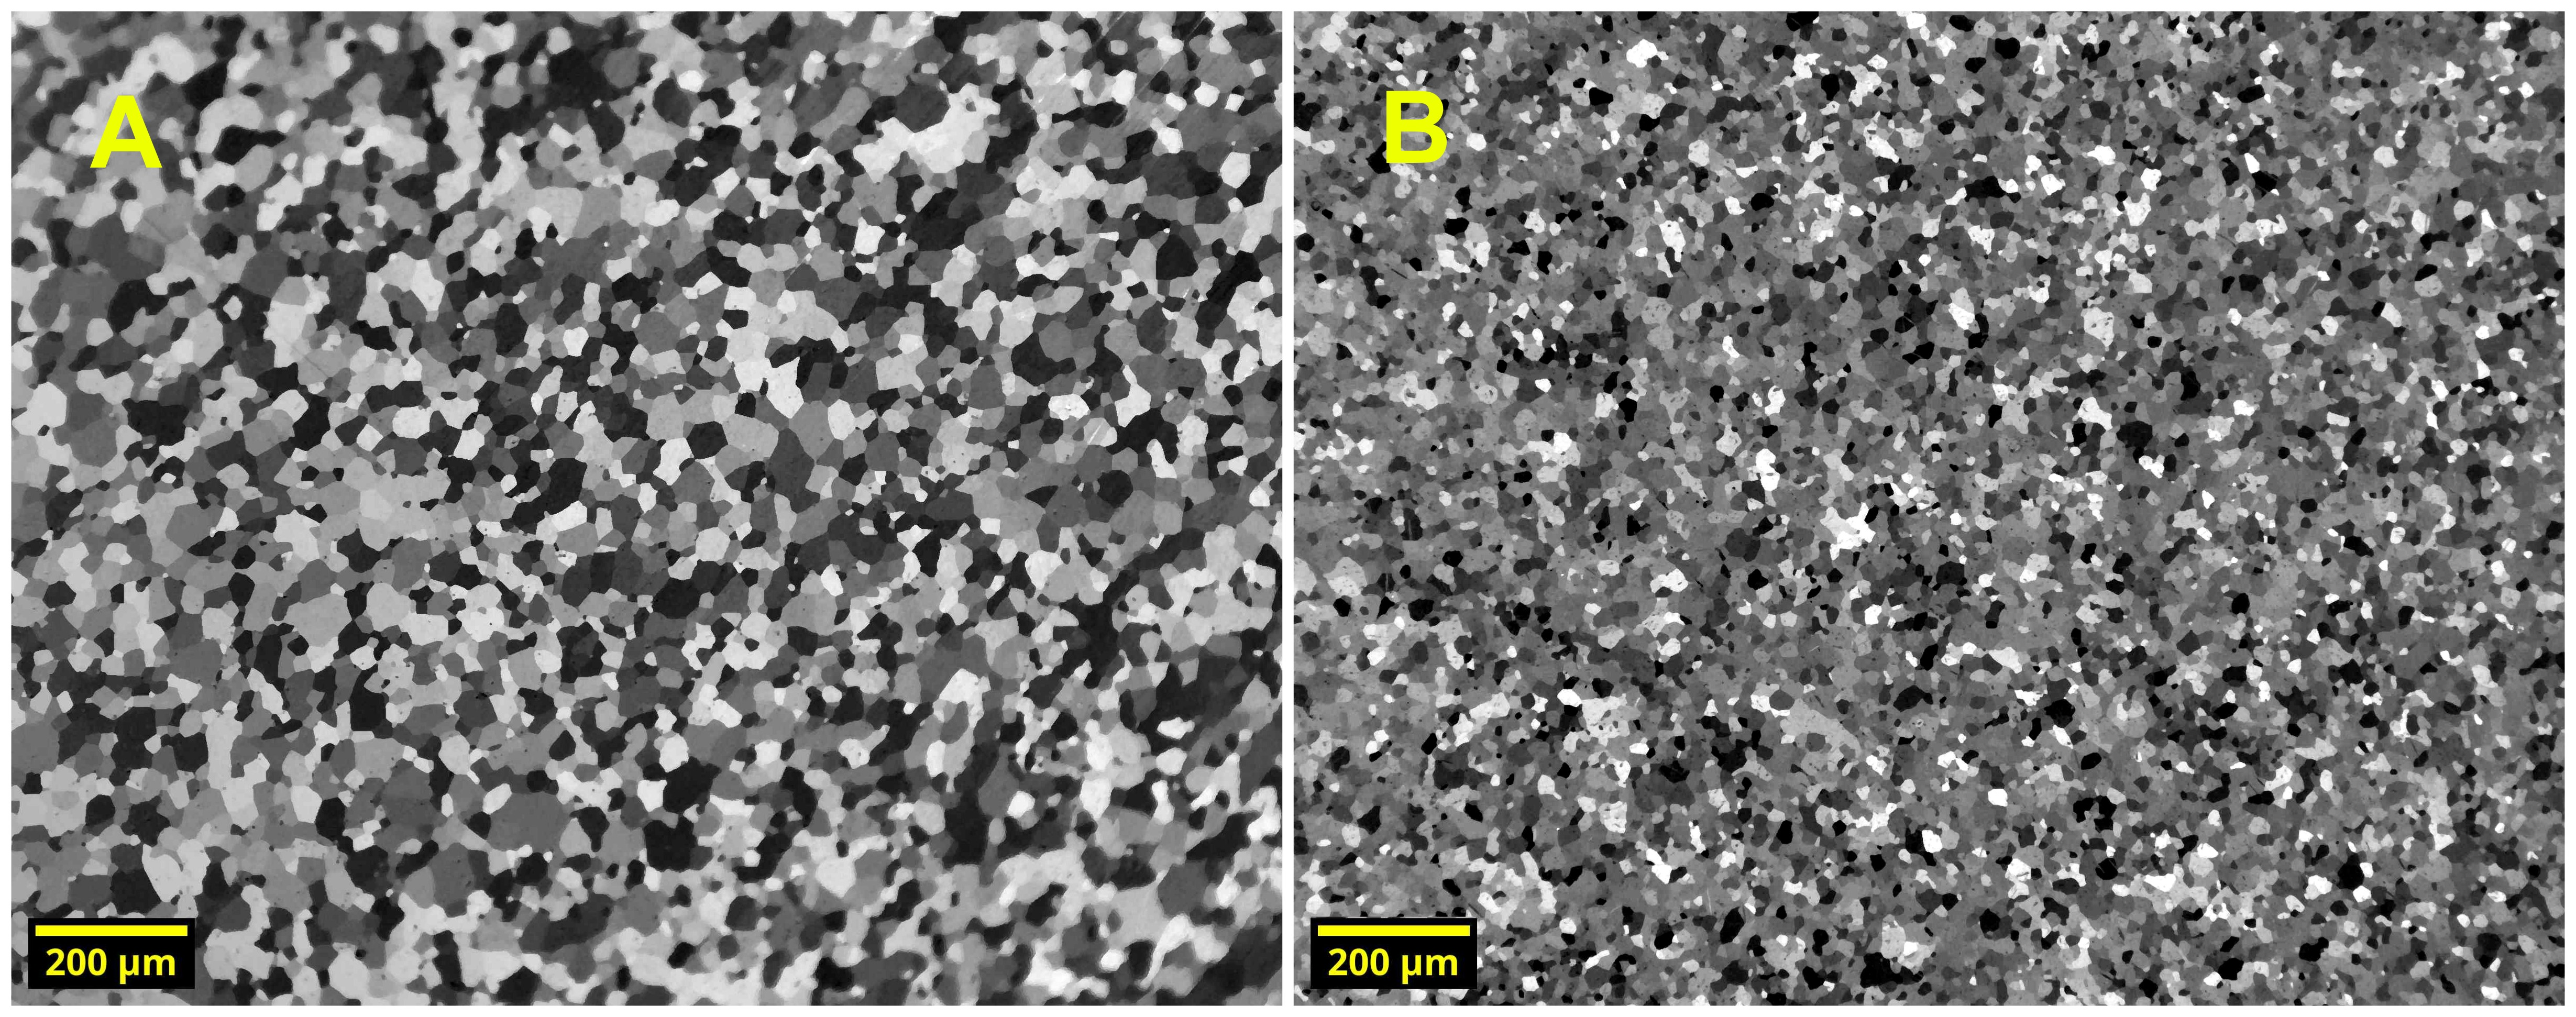
\includegraphics[width=\textwidth]{Figures/plate_sheet_OM.jpg}
  \caption{Polarised light optical micrograph of CP-Ti plate (A) and sheet (B). \label{fig.plateSheetOM}}
\end{figure}

\begin{figure}[h]
\centering
  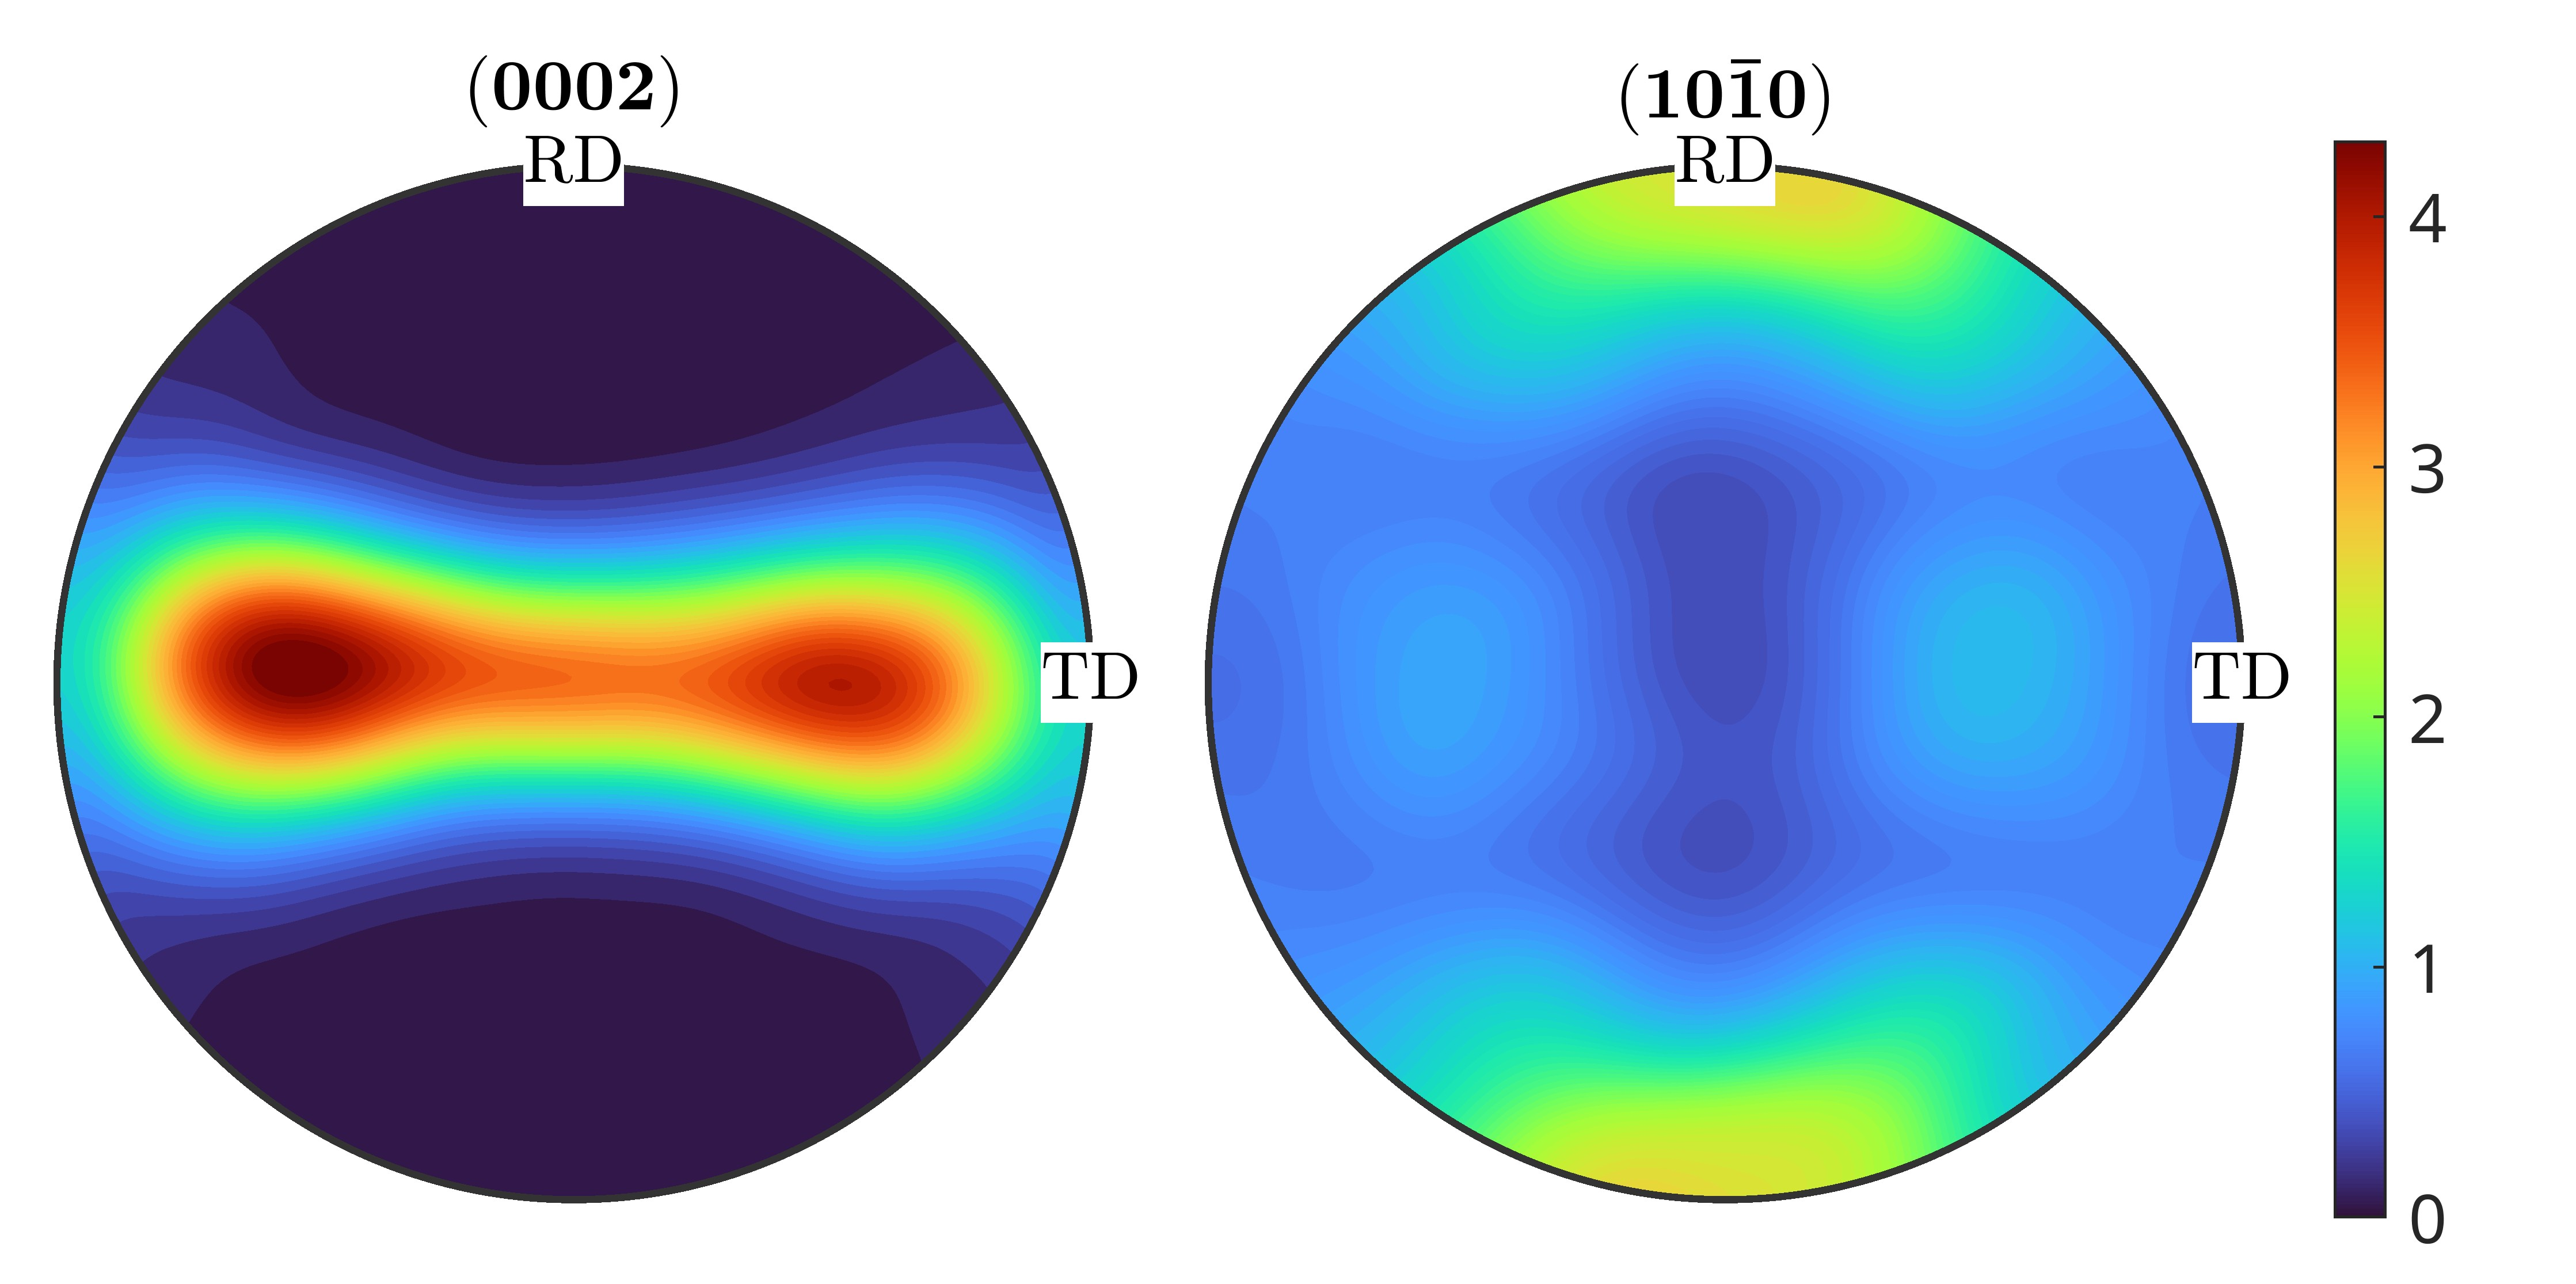
\includegraphics[width=\textwidth]{Figures/pf_plate_axisCorrectedjpg.jpg}
  \caption{Pole figures for CP-Ti plate, colour scale indicates multiples of random distribution. \label{fig.pfPlate}}
\end{figure}

Crystallographic texture measured with EBSD revealed a strong split basal texture in the CP-Ti plate, with a large TD split angle of approximately 45$^\circ$, as shown in \fref{fig.pfPlate}.
The large TD split is interesting because it exaggerates the already present anisotropy that is typical with a less pronounced TD split basal texture, with many grains having components of their $\langle c \rangle$-axis along TD but almost zero grains having $\langle c \rangle$-axis components along RD.

To examine the effect of such a strong texture, cylindrical samples along RD and TD were fabricated for tensile testing.
The results of tensile testing, shown in \fref{fig.tensilePlate}, reveal the significant anisotropy in mechanical response between the two primary plate directions.
The yield behaviour was completely different between both samples, with the RD sample undergoing a much earlier and smoother elastic-to-plastic transition.
For TD loading on the other hand, a much higher yield followed by a yield plateau was observed.

To quantify the early plasticity observed in the RD sample, the point where the stress-strain curves of the two samples diverge was determined.
The elastic limit was defined as the point when measurable plasticity in the RD sample had occurred.
The stress-strain data for both RD and TD was interpolated so that their stress difference at each strain point could be calculated by subtraction.
This difference function is plotted in \fref{fig.elasticLimit}.
During the elastic region, both samples behave very similarly and the difference remains flat.
This region was classified as the first 0.08\% strain, and the mean and standard deviation of the difference was determined.
Measurable plasticity was defined to be the point where the RD sample had deviated by more than 2 times the standard deviation, which occurred at a strain of 0.1\% and a stress of $111$MPa.

\begin{figure}[h!]
\centering
  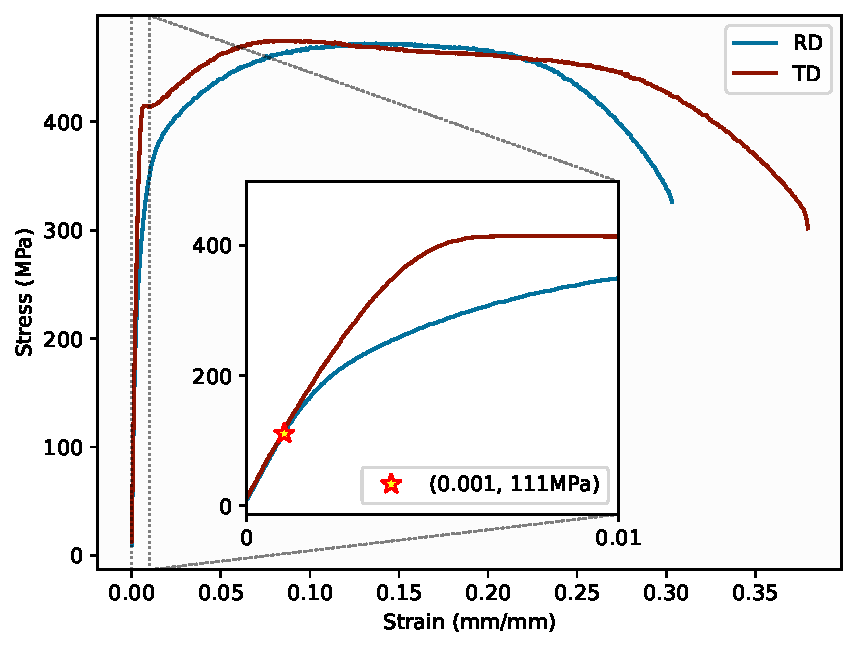
\includegraphics[width=\textwidth]{Figures/tensilePlotInset.pdf}
  \caption{Engineering stress-strain curve for CP-Ti for both rolling direction (RD) and transverse direction (TD). Elastic limit of RD sample marked on inset plot.\label{fig.tensilePlate}}
  \vspace{3\baselineskip}
  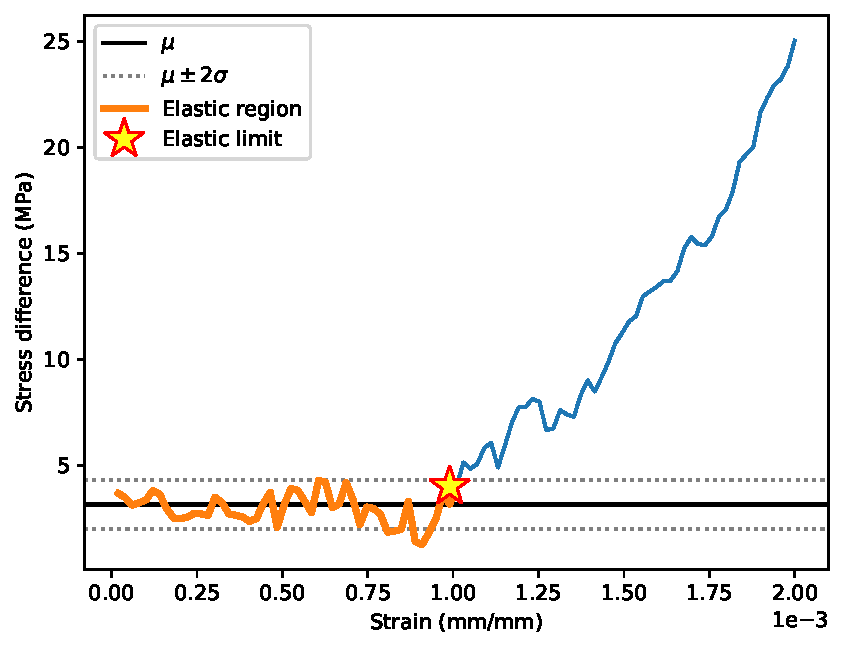
\includegraphics[width=0.6\textwidth]{Figures/elastic_limit.pdf}
  \caption{Stress difference ($\sigma_\textnormal{TD}-\sigma_\textnormal{RD}$) as a function of strain, revealing when the deformation behaviour diverges, indicating elastic limit of RD.\label{fig.elasticLimit}}
\end{figure}



\pagebreak
\section{HIP \#1: Abnormal grain growth}
The first HIP run appeared successful, and initial characterisation with EBSD revealed the desired microstructure of equiaxed $\alpha$ grains.
This initial characterisation however, was only conducted on a small part of the bottom of the HIP can.
Subsequent tensile testing results are shown in \fref{fig.tensileHIP}, in which strange load drop behaviour can be observed.
These load drops were accompanied by audible pings and were present in all 5 samples that were cut from the initial HIP can.
After some difficulty in explaining this phenomenon with respect to the assumed equiaxed microstructure, further characterisation of the material was made using cutoffs from the head sections of the tensile samples.

These cutoffs were etched using Kroll's reagent (1\% \ce{HF} + 4\% \ce{HNO3} + 95\% \ce{H2O}) and it was discovered that significant abnormal grain growth had occurred during the HIP, shown in \fref{fig.AGG}.
Very large grains can be seen which have grown to sizes on the order of several millimetres.
These grains appear to exist within a surviving matrix of normal grains which appear to be the same as the initially observed section of the HIP can, which did not present any abnormal grains.

The precise mechanism for the abnormal grain growth is not known.
It is known in the literature that the recrystallisation behaviour of alpha titanium is quite sensitive when held at high temperatures (but still beneath the beta-transus)\cite{tongFormationVeryLarge2017}.
Usually this phenomenon is related to recrystallisation after small strains, where the number density of recrystallisation nuclei may be quite small.
In such a regime, once recrystallisation nucleates, the new grain has unimpeded growth.
Provided that the small amount of work stored in the matrix is sufficient to support its growth, the new grain may grow to a very large size if there were no nearby recrystallisation nuclei.
The small strain in our case would be the initial plasticity required for consolidation of the powder.

In order to gain a deeper understanding and also as a second attempt at producing a fully random texture and consolidated HCP material, a second HIP was run using the two alternative powder stocks.
There was evidence of powder contamination in the original material, and therefore it was a plausible option to retry the same parameters with a different and hopefully uncontaminated powder.
The difference in powder size distribution would also change the dynamics of the early stage plasticity during consolidation and hopefully lead to a different result.


\begin{figure}[h]
\centering
  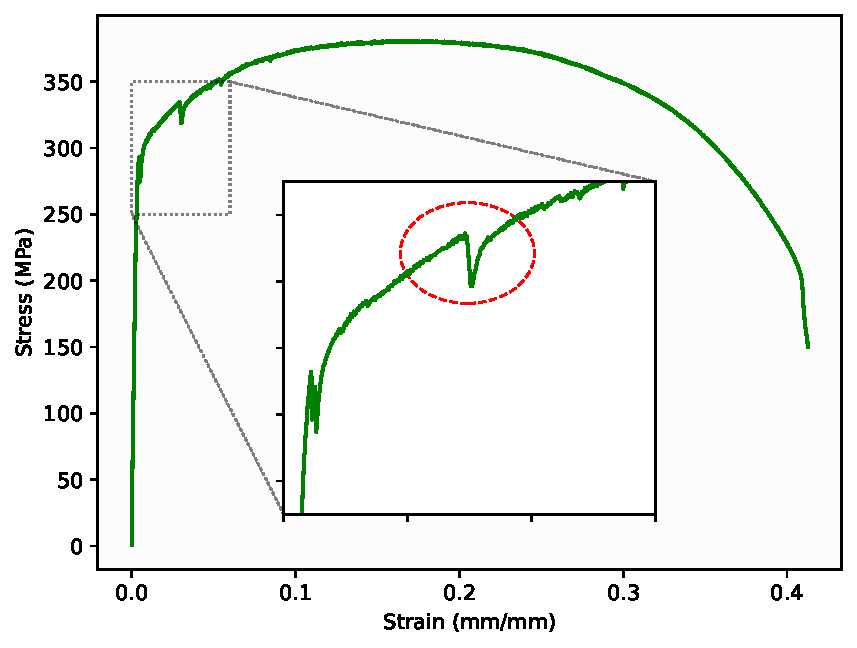
\includegraphics[width=\textwidth]{Figures/HIPtensile.pdf}
  \caption{Engineering stress-strain curve for HIP CP-Ti. Later discovered abnormal grain growth to be the cause of load drops. \label{fig.tensileHIP}}
  \vspace{\baselineskip}
  \includegraphics[width=\textwidth]{Figures/AGG.jpg}
  \caption{Optical micrograph of HIPed CP-Ti abnormal grain growth with Kroll's etch. \label{fig.AGG}}
\end{figure}


\section{HIP \#2: Success}

The second HIP trial was indeed successful, in both cases.
The two powder stocks that were used were the 45-90 $\mu$m (TLS powder) and the 53-100 $\mu$m (AVI powder). 
The resulting microstructure these cans had a grain size distribution of approximately 50 $\mu$m and 60 $\mu$m respectively (which may indicate that powder particle size is well correlated to final grain size).

The texture of the second HIP was quantified using EBSD large area measurements, which sampled many grains to generate pole figures, shown in \fref{fig.pfHIP}.
The same colour scale from \fref{fig.pfPlate} which highlights the sharp difference in texture strength.
Despite lacking any distinct texture features, the pole figure is not completely flat, which can be attributed to the sampling of a limited (though large) set of grains.

\begin{figure}[h!]
\centering
  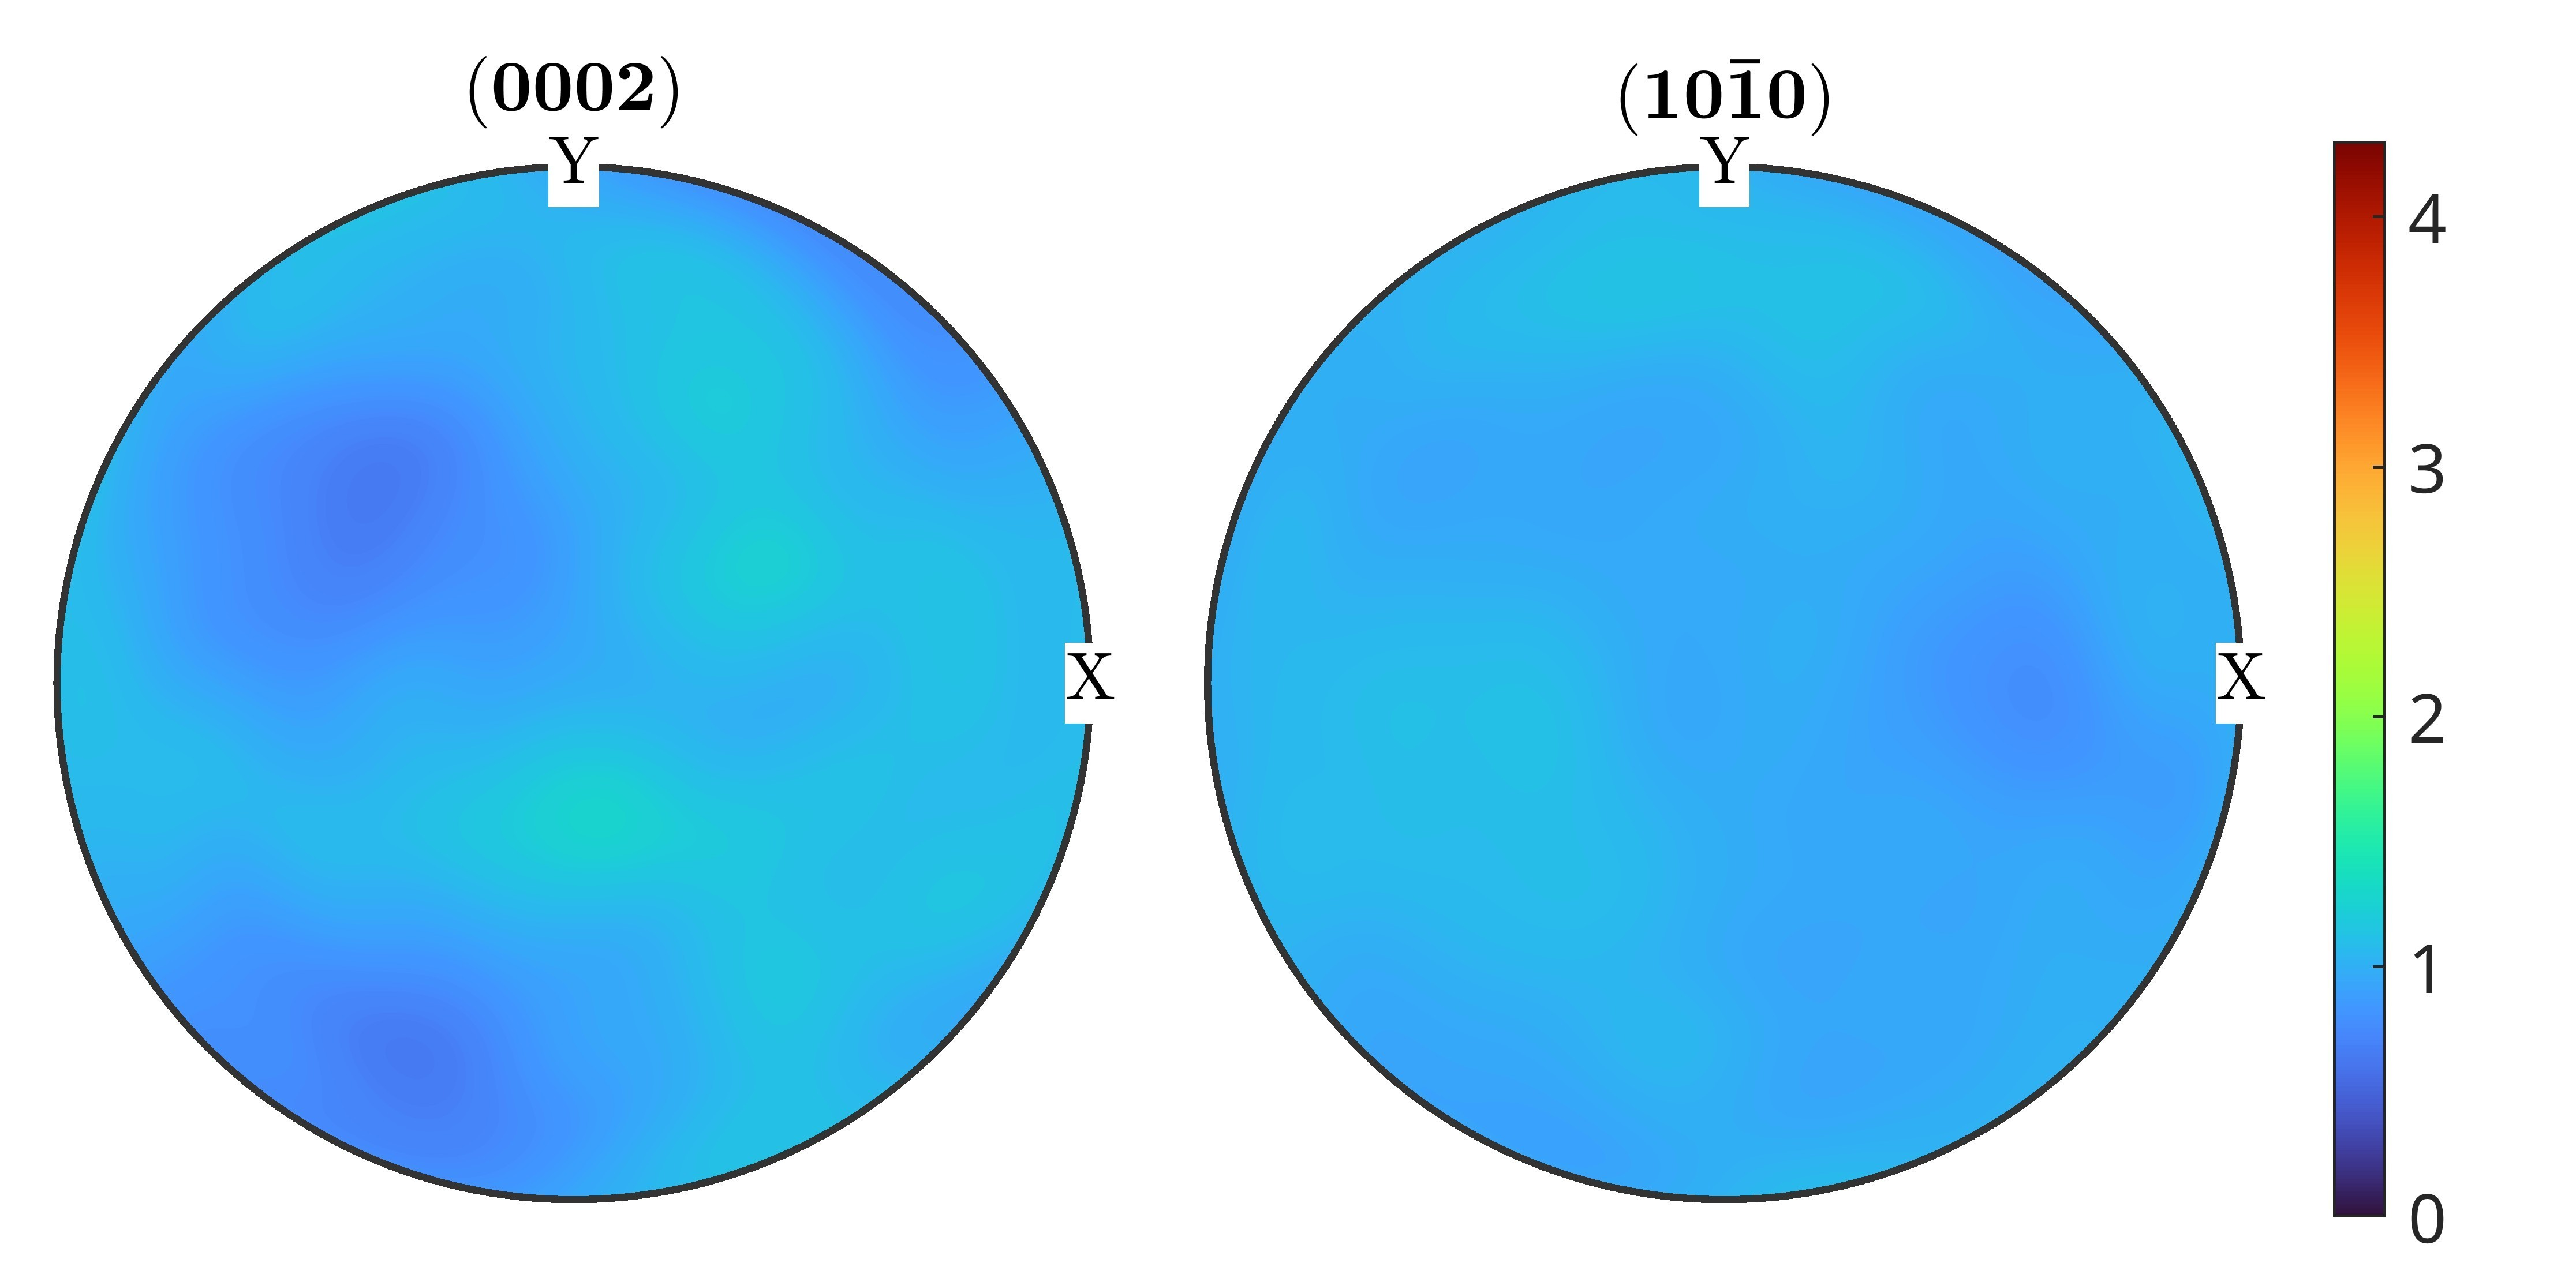
\includegraphics[width=\textwidth]{Figures/pf_HIP_TLS.jpg}
  \caption{Pole figures for HIPed CP-Ti using same colour scale as \fref{fig.pfPlate}.\label{fig.pfHIP}}
  \vspace{\baselineskip}
  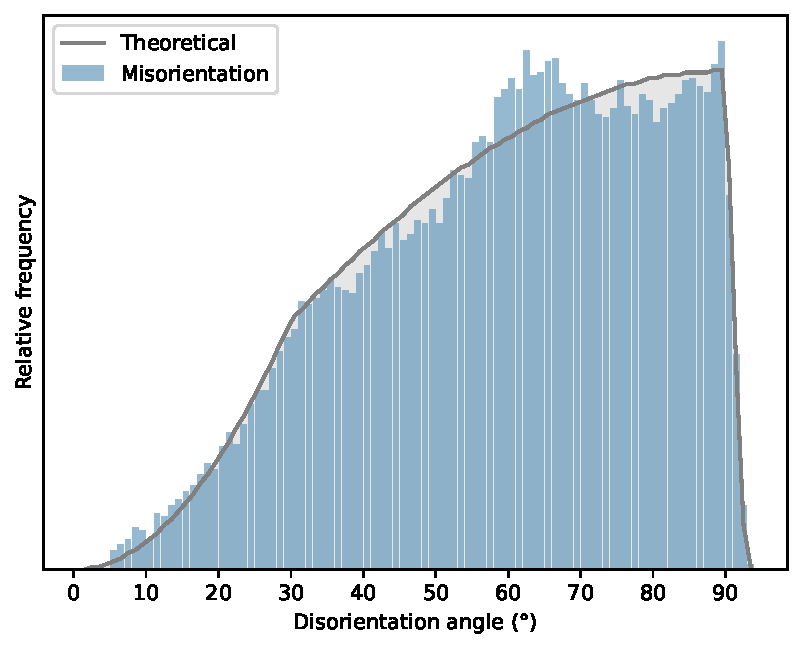
\includegraphics[width=0.7\textwidth]{Figures/disorientationDist.pdf}
  \caption{Disorientation distribution for HIP\#2, agreement with theoretical distribution for random texture.\label{fig.disorientationPlot}}
\end{figure}

The random-texture can further be quantified using the three Kearns factors: 0.3363, 0.3249, 0.3388.
For a theoretically random texture, the Kearns factors are each exactly 1/3.
Finally, the disorientation plot in \fref{fig.disorientationPlot} shows a very close agreement to the theoretical Mackenzie plot for a truly random orientation distribution.
It is therefore concluded that HIPing has proved a successful technique for producing randomly textured HCP microstructures.


\subsection{Geometric compatibility}
EBSD maps were used to calculate the grain neighbour compatibility in both the HIPed material and the conventionally rolled material.
First, a global loading condition along RD was assumed, which allowed Schmid factor analysis to be used to determine the active slip system in each grain.
Only prismatic slip systems were considered for this preliminary analysis.
Once the active slip systems were identified, for each neighbouring pair, the Luster-Morris parameter $m'$ was calculated across their boundary to determine how well the pair can accommodate slip between them.
A map of these $m'$ values in the HIP material is shown in \fref{fig.mPrimeMap}, where brighter colours represent boundaries most likely to be sites for slip transfer events.

A statistical representation of the $m'$ values is shown by the histogram in \fref{fig.mPrimeHist}.
A distinct peak at the high end of $m'$ values is present in the rolled material which is completely absent in the HIPed material.
A typical threshold for direct slip transfer is $m' > 0.8$ \cite{nieto-valeirasAnalysisSlipTransfer2024}.
In the rolled sample, 19\% fo grain boundaries are above this threshold, compared to only 7\% in the HIPed sample.
There is a measurable difference in the geometric alignment of neighbouring grains, which can be explained by the rolled texture having a more restricted set of possible grain orientations due to many orientations being absent from the orientation distribution (e.g. almost zero grains with c-axis aligned with RD).
This means that grains are more likely to have similar orientations with their neighbours and this is reflected in the peak at higher $m'$ values.

If polycrystalline strain localisation can be considered as a networking phenomenon, then a description based on percolation theory may be suitable.
The extent of networks of geometrically aligned grains would then be dependent on the expected fraction of neighbouring grains that have good alignment.


\begin{figure}[ht]
\centering
  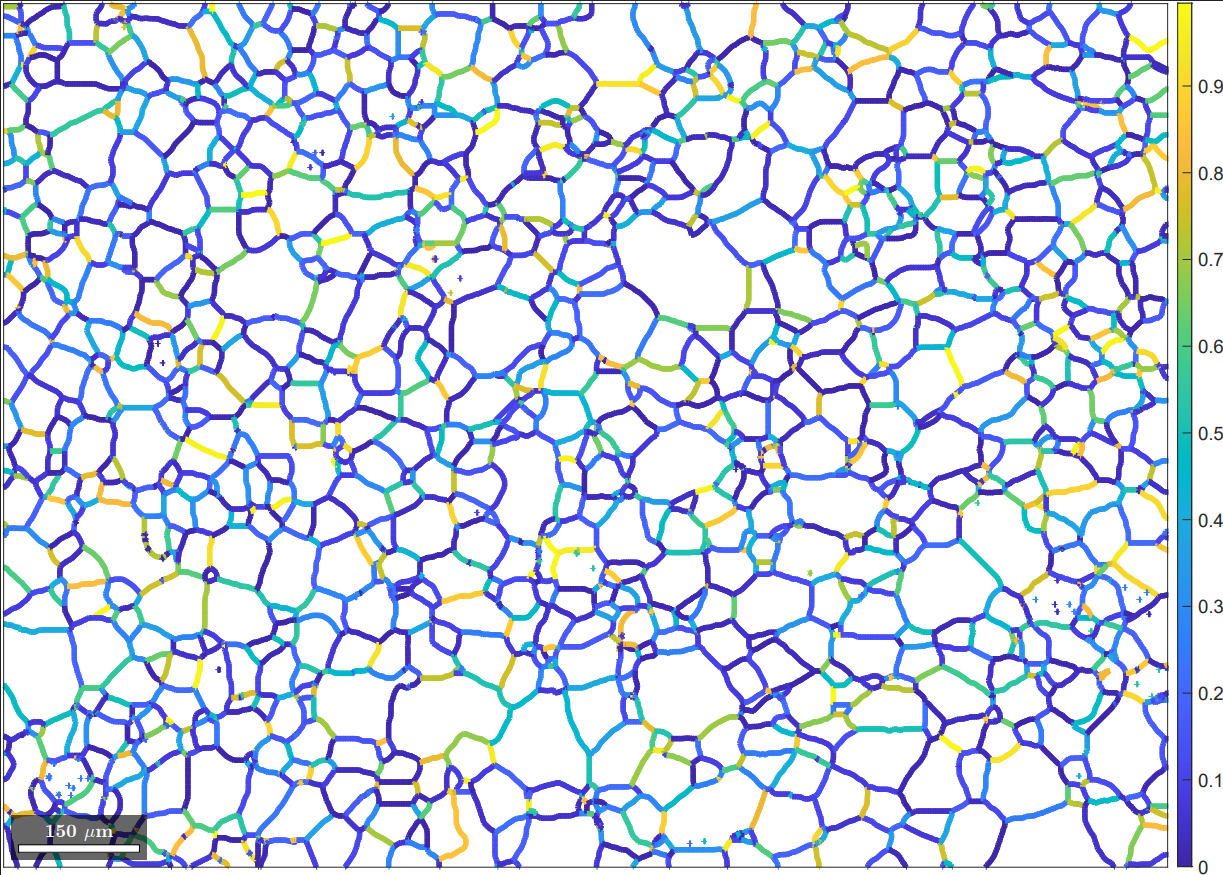
\includegraphics[width=\textwidth]{Figures/mPrimeMap_HIP.png}
  \caption{Map of $m'$ values in HIPed CP-Ti.\label{fig.mPrimeMap}}
  \vspace{\baselineskip}
  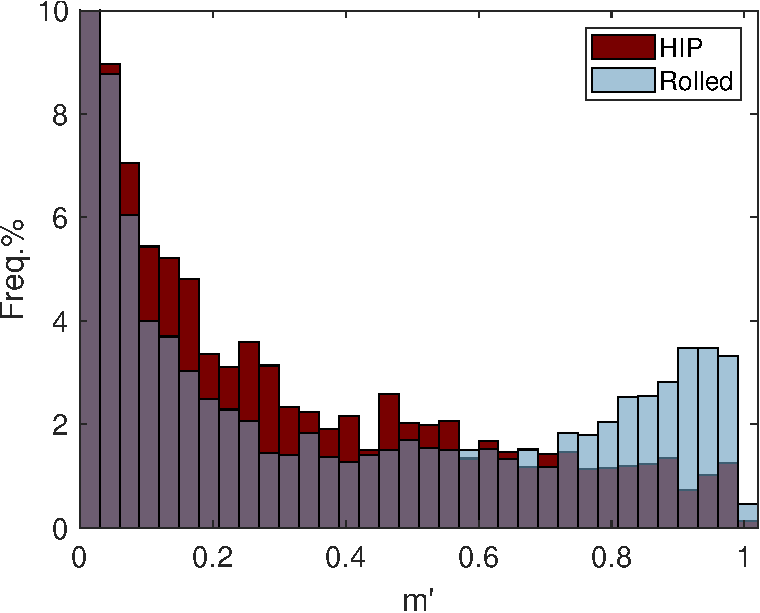
\includegraphics[width=0.8\textwidth]{Figures/mPrimeHistogram.pdf}
  \caption{Histogram of $m'$ values for rolled (RD loading) and HIPed CP-Ti.\label{fig.mPrimeHist}}
\end{figure}